\documentclass{beamer}

\newcommand\unit{0.75}
\newcommand\zero{0}
\newcommand\one{\unit}
\newcommand\two{2 * \unit}

\newcommand\aunit{0.75}

\usepackage{appendixnumberbeamer}

\usepackage{tikz}
\usetikzlibrary{positioning}
\tikzset{box/.style={rectangle,draw=black,thick, minimum size=\unit cm}}

\usepackage{amsfonts}
\usepackage{amsmath}
\usepackage{amsthm}
\usepackage{amssymb}
\usepackage{mathdots}
\usepackage{stmaryrd}
\usepackage{datetime}

\DeclareMathOperator*{\argmax}{argmax}

% images
\usepackage{graphicx}
\graphicspath{ {./images} }

\usepackage{caption}
\usepackage{subcaption}

\tikzset{
    hsvipomdp/.pic={
        \draw[black, thick] (-3.5*\aunit, 0*\aunit) -- node[midway,below]{$\Delta(S)$} (3.5*\aunit, 0*\aunit);
        \draw[black, thick] (-3*\aunit, -0.5*\aunit) -- (-3*\aunit, 3*\aunit);
        \draw[black, thick] (3*\aunit, -0.5*\aunit) -- (3*\aunit, 3*\aunit);
        \draw[black] plot[smooth, domain=-3*\aunit:3*\aunit] (\x, {((\x - 0.5*\aunit)^2) / 10*\aunit + 0.85*\aunit});
        \draw[black, dotted] (-3*\aunit, 2.5*\aunit) -- (3*\aunit, -0.5*\aunit);
        \draw[black, dotted] (-3*\aunit, 1.5*\aunit) -- (3*\aunit, 1*\aunit);
        \draw[black, dotted] (-3*\aunit, 0.5*\aunit) -- (3*\aunit, 1.5*\aunit);
        \draw[black, dashed] (-3*\aunit, 2.5*\aunit) -- (-0.6*\aunit, 1.3*\aunit);
        \draw[black, dashed] (-0.6*\aunit, 1.3*\aunit) -- (1*\aunit, 1.16*\aunit);
        \draw[black, dashed] (1*\aunit, 1.16*\aunit) -- (3*\aunit, 1.5*\aunit);
        \filldraw[black] (-0.6*\aunit, 1.3*\aunit) circle (1pt);
        \filldraw[black] (1*\aunit, 1.16*\aunit) circle (1pt);
        \filldraw[black] (-3*\aunit, 2.5*\aunit) circle (1pt);
        \filldraw[black] (3*\aunit, 1.5*\aunit) circle (1pt);
        \draw[black, dotted] (-3*\aunit, 1*\aunit) -- (3*\aunit, 0*\aunit);
        \draw[black, dotted] (-3*\aunit, 0.6*\aunit) -- (3*\aunit, 0.6*\aunit);
        \draw[black, dotted] (-3*\aunit, 0*\aunit) -- (3*\aunit, 0.8*\aunit);
        \draw[black, very thick] (-3*\aunit, 1*\aunit) -- (-0.6*\aunit, 0.6*\aunit);
        \draw[black, very thick] (-0.6*\aunit, 0.6*\aunit) -- (1.5*\aunit, 0.6*\aunit);
        \draw[black, very thick] (1.5*\aunit, 0.6*\aunit) -- (3*\aunit, 0.8*\aunit);
        \draw (-3*\aunit, 2.5*\aunit - 1*\aunit) node[anchor=east]{\tiny $V^*$};
        \draw (-3*\aunit, 2.5*\aunit) node[anchor=east]{\tiny $V_{UB}$};
        \draw (-3*\aunit, 1*\aunit) node[anchor=east]{\tiny $V_{LB}$};
    }
}

\usetheme{metropolis}
\metroset{block=fill, numbering=fraction}
\setbeamertemplate{navigation symbols}{}

\title[Comparing Exploration Methods in POSGs]{Comparing Exploration Methods in Partially Observable Stochastic Games}
\author{Jakub Rada}
\institute{
    Faculty of Electrical Engineering
    \\
    Czech Technical University in Prague
}
\usdate
\newdate{date}{14}{06}{2022}
\date{\displaydate{date}}

\begin{document}
\frame{\titlepage}

\section{Motivation and multi-armed bandits}

\begin{frame}{Motivation}
\begin{itemize}
    \item SGs and POSGs have applications in economy, stock markets, network security, biology, machine learning, etc.
    \item solving algorithms exist, but often require linear programming 
    \begin{itemize}
        \item value iteration, HSVI
    \end{itemize}
    \item multi-armed bandits can be used as an alternative approach of exploring the search space
\end{itemize}
\end{frame}

\begin{frame}{Multi-armed bandits}
Stochastic bandit algorithms
\begin{itemize}
    \item Best of $N$, $\epsilon$-greedy
    \item Successive Elimination, UCB
    \item \textbf{observable} variants for each of the above - only in SGs
\end{itemize}
Adversarial bandits
\begin{itemize}
    \item Exp3
\end{itemize}
\end{frame}

\section{Stochastic Games}

\begin{frame}{SG model}
    \begin{block}{Stochastic game}
        A \textit{stochastic game} is a tuple $G = \left(S, A_1, A_2, T, R, \gamma\right)$, where
        \begin{itemize}
            \item $S$ is a set of states of the game,
            \item $A_1$, $A_2$ are sets of actions available to player 1, resp. player 2,
            \item $T: S \times A_1 \times A_2 \times S \to \left[0, 1\right]$ is a transition function,
            \item $R: S \times A_1 \times A_2 \to \mathbb{R}$ is a reward function and
            \item $\gamma \in \left(0, 1\right)$ is the discount factor.
        \end{itemize}
    \end{block}
    \begin{columns}
        \column{0.5\textwidth}
        \begin{flushright}
            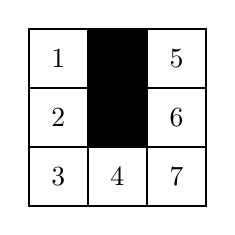
\begin{tikzpicture}
                \foreach \x in {\zero,\one,\two}{\foreach \y in {\zero,\one,\two}\node[box] at (\x,\y){};}
                \node[box] at (\zero, \two) {1};
                \node[box, fill=black] at (\one, \two) {};
                \node[box] at (\two, \two) {5};

                \node[box] at (\zero, \one) {2};
                \node[box, fill=black] at (\one, \one) {};
                \node[box] at (\two, \one) {6};

                \node[box] at (\zero, \zero) {3};
                \node[box] at (\one, \zero) {4};
                \node[box] at (\two, \zero) {7};
            \end{tikzpicture}
        \end{flushright}
        \column{0.5\textwidth}
        \begin{flushleft}
            Example map of a stochastic game \textbf{Tag}
        \end{flushleft}
    \end{columns}
\end{frame}

\begin{frame}{Value iteration for SGs}
    \begin{itemize}
        \item based on a value function $V: S \to \mathbb{R}$
        \item starts from initial $V^0$
        \item iterative application of a Bellman operator refines the approximation $V^t$ to $V^{t+1}$
        \begin{block}{Stage game $u$ for a state $s \in S$}
            \setlength\abovedisplayskip{0pt}
            \begin{multline*}
                \forall a_1 \in A_1, \forall a_2 \in A_2: \\
                u(a_1, a_2) = R(s, a_1, a_2) + \gamma \sum_{s^{\prime}}T(s^{\prime} | s, a_1, a_2) \cdot V(s^{\prime})
            \end{multline*}
        \end{block}
        \item stage game can be replaced by some bandit algorithm
        \item terminates when $|V^t(s) - V^{t+1}(s)| \leq \epsilon \quad \forall s \in S$
    \end{itemize}
\end{frame}

\begin{frame}{Comparison on SG}
    \begin{figure}
        \centering
        \includegraphics[width=1\textwidth]{./tag_3_01_EpsilonGreedy_UCB_ObservableEpsilonGreedy_ObservableUCB_Exp3_LinT_3_3.png}
        \caption{Best bandit algorithms in a state with mixed optimal strategies}
    \end{figure}
\end{frame}

\section{One-Sided Partially Observable Stochastic Games}

\begin{frame}{OS-POSG model}
    \begin{block}{One-sided partially observable stochastic game}
        An \textit{OS-POSG} is a tuple $G = \left(S, A_1, A_2, O, T, R, b^{\text{init}}, \gamma\right)$, where $S$, $A_1$, $A_2$, $R$, $\gamma$ are the same as in SGs and
        \begin{itemize}
            \item $O$ is a set of private observations for player 1,
            \item $T: S \times A_1 \times A_2 \times O \times S \to \left[0, 1\right]$ is a transition function,
            \item $b^{\text{init}} \in \Delta(S)$ is an initial belief over states in $S$.
        \end{itemize}
    \end{block}
    \begin{columns}
        \column{0.25\textwidth}
        \begin{flushright}
            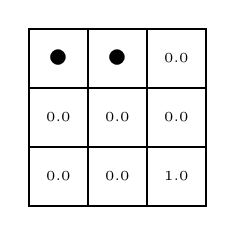
\begin{tikzpicture}
                \foreach \x in {\zero,\one,\two}{\foreach \y in {\zero,\one,\two}\node[box] at (\x,\y){};}
                \node[box] at (\zero, \two) {\Large$\bullet$};
                \node[box] at (\one, \two) {\Large$\bullet$};
                \node[box] at (\two, \two) {\tiny 0.0};

                \node[box] at (\zero, \one) {\tiny 0.0};
                \node[box] at (\one, \one) {\tiny 0.0};
                \node[box] at (\two, \one) {\tiny 0.0};

                \node[box] at (\zero, \zero) {\tiny 0.0};
                \node[box] at (\one, \zero) {\tiny 0.0};
                \node[box] at (\two, \zero) {\tiny 1.0};
            \end{tikzpicture}
        \end{flushright}
        \column{0.25\textwidth}
        \begin{flushright}
            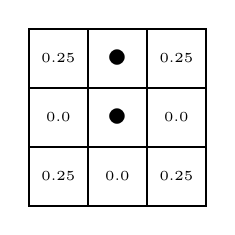
\begin{tikzpicture}
                \foreach \x in {\zero,\one,\two}{\foreach \y in {\zero,\one,\two}\node[box] at (\x,\y){};}
                \node[box] at (\zero, \two) {\tiny 0.25};
                \node[box] at (\one, \two) {\Large$\bullet$};
                \node[box] at (\two, \two) {\tiny 0.25};

                \node[box] at (\zero, \one) {\tiny 0.0};
                \node[box] at (\one, \one) {\Large$\bullet$};
                \node[box] at (\two, \one) {\tiny 0.0};

                \node[box] at (\zero, \zero) {\tiny 0.25};
                \node[box] at (\one, \zero) {\tiny 0.0};
                \node[box] at (\two, \zero) {\tiny 0.25};
            \end{tikzpicture}
        \end{flushright}
        \column{0.5\textwidth}
        \begin{flushleft}
            Example initial setting of an OS-POSG \textbf{Pursuit-Evasion}

            \vspace*{1em}

            \begin{tabular}{c c l}
                {\Large $\bullet$} & $\dots$ & Pursuer units \\
                {\tiny $p$} & $\dots$ & probability of Evader
            \end{tabular}
        \end{flushleft}
    \end{columns}
\end{frame}

\begin{frame}{HSVI for OS-POSGs}
    \begin{itemize}
        \item two bounding value functions: $V_{LB} \leq V^* \leq V_{UB}$
        \begin{itemize}
            \item values are computed against opponent's \textit{best response}
        \end{itemize}
        \item iterative application of the Bellman operator pushes the bounds closer together
        \item terminate when $V_{UB}(b^{\text{init}}) - V_{LB}(b^{\text{init}}) \leq \epsilon \quad \epsilon \in (0, +\infty)$
        \item the LP performing the update can be replaced by any of the bandits
    \end{itemize}
    \begin{center}
        \tikz\pic{hsvipomdp};
    \end{center}
\end{frame}

\begin{frame}{Comparison on OS-POSG}
    \begin{figure}
        \centering
        \includegraphics[width=0.9\textwidth]{./easier_discount_095.png}
        \caption{Dependence of the values in $b^{\text{init}}$ on number of bound updates. Bounding value functions approach the optimal value.}
    \end{figure}
\end{frame}

\begin{frame}{Conclusion}
    \begin{itemize}
        \item successfully integrated and compared multi-armed bandit algorithms into value iteration and HSVI
        \item \textbf{observable} variants consistently better than standard bandits (on SGs)
        \item Exp3 performs well on both models
        \item ObservableUCB usually same or better than Exp3 (on SGs)
        \item high exploration is important in HSVI
        \item Successive elimination, Best of N and standard UCB rarely get close to the optimal value
    \end{itemize}
\end{frame}

\begin{frame}
    Thank you for your attention
\end{frame}

\appendix

\begin{frame}{"Averaging" factor}
    A method used in SGs to compute refined value function:
    \begin{equation*}
        V^{t+1}(s) = V^{t}(s) + \delta(t) \cdot (v - V^{t}(s)),
    \end{equation*}
    where $v$ is the immediate value from current iteration and $\delta(t)$ one of the following functions of time $t$:
    \begin{itemize}
        \item $\delta(t) = \frac{1}{t}$ 
        \item $\delta(t) = \frac{1}{\sqrt{t}}$ 
    \end{itemize}

    Parametrisation and adaptive fitting?
\end{frame}

\begin{frame}{Suggestions}
    \begin{equation*}
        V^{t+1}(s) = V^{t}(s) + \delta(t) \cdot (v - V^{t}(s))
    \end{equation*}
    Parametrisation
    \begin{itemize}
        \item $\delta(t, a) = t^{-\frac{1}{a}} \qquad a > 0$
        \item hyperparameter $a$ can be tuned for each problem separately
    \end{itemize}
    Adaptive fitting
    \begin{itemize}
        \item gradually decrease the $\delta(t)$ factor in time
        \begin{itemize}
            \item at the beggining faster changes in value are beneficial
            \item towards the end decrease $\delta(t)$ to prevent fluctuations caused by exploring bandits
            \item linear decay, exponential decay from some initial setting
        \end{itemize}
        \item set $\delta(t)$ based on $d = |v - V^t(s)|$
        \begin{itemize}
            \item $d$ grows $\rightarrow$ decrease $\delta(t)$ (towards i.e. $\frac{1}{t}$)
            \item $d$ gets smaller $\rightarrow$ increase $\delta(t)$ (towards i.e. $\frac{1}{\sqrt{t}}$)
        \end{itemize}
    \end{itemize}
\end{frame}

\begin{frame}{Suggestions (HSVI)}
    Similar idea for HSVI
    \begin{itemize}
        \item monitor progress of gap $g = V_{UB}(b^{\text{init}}) - V_{LB}(b^{\text{init}})$
        \item if the decrease of $g$ starts to be slow $\rightarrow$ increase exploration
    \end{itemize}
\end{frame}

\end{document}
